\documentclass[11pt]{article}
\usepackage[margin=0.9in]{geometry}
\usepackage{booktabs,graphicx,float,amsmath,xcolor,enumitem}
\usepackage[hidelinks]{hyperref}
\usepackage{titlesec}
\titleformat{\section}{\large\bfseries}{\thesection.}{0.5em}{}
\titleformat{\subsection}{\normalsize\bfseries}{}{0em}{}
\titlespacing*{\section}{0pt}{8pt}{3pt}
\titlespacing*{\subsection}{0pt}{8pt}{2pt}
\setlength{\parindent}{0pt}
\setlength{\parskip}{4pt}
\setlist{nosep,leftmargin=1.2em}
\setlist[itemize]{label=\textbullet}
\newcommand{\taurct}{\hat\tau^{\,\mathrm{RCT}}}
\newcommand{\taunaive}{\hat\tau^{\,\mathrm{naive}}}

\begin{document}

\begin{center}
{\Large\bfseries Do City Chiefs Grant More Discretionary Tax Exemptions?}

\vspace{4pt}
\textbf{Name:} Tsu Ning Tsao \quad \textbf{Student Number:} 1012713137
\end{center}

\textbf{Research summary.} When neighbourhood chiefs (Local) instead of state agents (Central) collect the property tax, do more properties get exempted, and are the extra exemptions justified by the owner's legal status or discretionary favours? \textbf{Data:} replication data of Bal\'an et al.\ (2022), 2018 property-tax campaign in Kananga, D.R.\ Congo; neighbourhoods (\texttt{a7}) were randomly assigned to Central (\texttt{tmt}=1) or Local (\texttt{tmt}=2); the unit is the property. \textbf{Variables:} outcome $Y$ = \texttt{exempt} (1 if the collector registered the property as exempt); treatment $D$ = \texttt{local}; selection variable $S$ = owner age; other pre-treatment covariates $X$ = female, Luluwa (main tribe), works for the state.

\textbf{Track: RCT. Dataset:} the \textbf{biased sample} from Week 6 (Recipe B, $\alpha=0$, $\gamma=1$, $S$ = owner age, seed 1465; 2,740 properties in 192 neighbourhoods, 1,412 Local and 1,328 Central) unless a row or caption says ``Full'' (full experimental sample, 5,645 properties in 202 neighbourhoods). Code: \texttt{Week9/00\_master/00\_master.py} $\rightarrow$ \texttt{02\_analysis/02\_week9\_doubly\_robust.py}; outputs in \texttt{03\_output/week9/}.

\section{Doubly robust models (biased sample)}

\subsection{Step 1: The doubly robust model and its two components}
\begin{itemize}
\item \textbf{Estimator.} AIPW with cross-fitting (\texttt{econml.dr}). For each property, the pseudo-outcome is
$\psi_i=\hat\mu_1(x_i)-\hat\mu_0(x_i)+\frac{D_i\,(Y_i-\hat\mu_1(x_i))}{\hat e(x_i)}-\frac{(1-D_i)\,(Y_i-\hat\mu_0(x_i))}{1-\hat e(x_i)}$, and the ATE is its mean. The estimate is consistent if \emph{either} the outcome model or the propensity model is right. Covariates: $S$ and $X$.
\item \textbf{Outcome model} $\hat\mu_d(x)=E[Y\mid D=d,x]$: gradient-boosted trees (\texttt{GradientBoostingRegressor}, learning rate 0.05). A small grid chosen by CV picked depth 3, 100 trees and at least 100 properties per leaf, the same as in Week 8 (Table~1).
\item \textbf{Propensity model} $\hat e(x)=\Pr(D=1\mid x)$: logistic regression, the Week 7 logit. It has a lower CV log loss than a boosted classifier (0.603 vs 0.606). It is also the right functional form here: Recipe B selects on a logistic function of $S$.
\item \textbf{Cross-fitting.} 5 folds formed by neighbourhood (\texttt{GroupKFold}). Each property's $\hat\mu$ and $\hat e$ come from models that did not see its neighbourhood. Five folds train each nuisance model on 80\% of the data. Grouping matters because exemptions are correlated within a neighbourhood: random folds would leak information and make the nuisances look better than they are.
\end{itemize}
\begin{table}[H]\centering\small
\caption{Choosing the nuisance models: 5-fold CV by neighbourhood, biased sample, covariates $S$ and $X$.}
\begin{tabular}{llr}
\toprule
Model & Learner & CV loss \\
\midrule
Outcome (MSE) & GBR depth 3, 100 trees, leaf 100 (chosen) & 0.1546 \\
Outcome (MSE) & OLS (linear in S, X, D) & 0.1601 \\
Outcome (MSE) & Constant (mean) & 0.2205 \\
Propensity (Log loss) & Logit on S, X (Week 7) (chosen) & 0.6028 \\
Propensity (Log loss) & Gradient-boosted classifier & 0.6063 \\
Propensity (Log loss) & Constant (share Local) & 0.6927 \\
\bottomrule
\end{tabular}

\par\smallskip\footnotesize GBR grid: depth $\{2,3\}$ $\times$ trees $\{100,200\}$ $\times$ min leaf $\{50,100\}$; only the best of the 8 is shown (all lie between 0.1546 and 0.1558; full grid in \texttt{table1\_nuisance\_cv.csv}).
\end{table}

\subsection{Step 2: Validation (overlap and four EconML DR learners)}
\begin{figure}[H]\centering
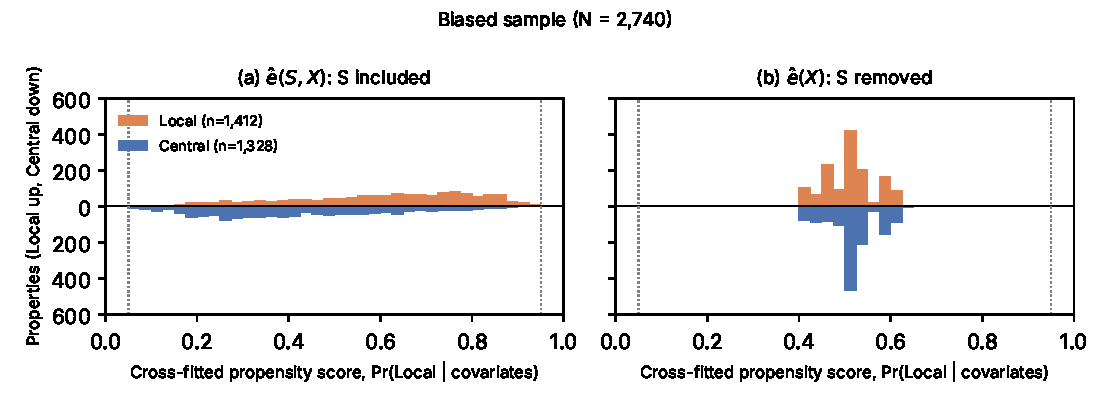
\includegraphics[width=\linewidth]{figure1_overlap.pdf}
\caption{Cross-fitted propensity scores, biased sample. (a) Covariates $S$ and $X$ (main model). (b) $S$ removed, $X$ only (Step 3). Dotted lines at 0.05 and 0.95.}
\end{figure}
\textbf{Overlap holds} (panel a). The cross-fitted scores run from 0.05 to 0.95. No property lies outside $[0.05, 0.95]$, 2.5\% lie outside $[0.10, 0.90]$, and the largest implied IPW weight is 14.7. This is the same picture as Week 7: Local properties sit at high scores (older owners), but both groups appear across the whole range. So the $1/\hat e$ terms in $\psi$ stay bounded and no trimming is needed.

\begin{table}[H]\centering\small
\caption{Doubly robust ATE of Local on \texttt{exempt}, biased sample ($N=2{,}740$): four EconML DR learners plus one nuisance swap, with $S$ included and with $S$ removed.}
\resizebox{\linewidth}{!}{\begin{tabular}{lcccc}
\toprule
 & \multicolumn{2}{c}{S included (covariates S, X)} & \multicolumn{2}{c}{S removed (X only)} \\
\cmidrule(lr){2-3}\cmidrule(lr){4-5}
DR learner & ATE (SE) & 95\% CI & ATE (SE) & 95\% CI \\
\midrule
DRLearner, GBR final stage & 0.039 (0.031) & [-0.041, 0.092] & 0.204 (0.036) & [0.129, 0.274] \\
LinearDRLearner (main) & 0.039 (0.031) & [-0.041, 0.092] & 0.204 (0.036) & [0.129, 0.274] \\
SparseLinearDRLearner & 0.039 (0.031) & [-0.041, 0.092] & 0.204 (0.036) & [0.129, 0.274] \\
ForestDRLearner & 0.040 (0.031) & [-0.042, 0.095] & 0.202 (0.036) & [0.131, 0.277] \\
LinearDRLearner, random-forest nuisances & 0.039 (0.032) & [-0.039, 0.094] & 0.203 (0.036) & [0.130, 0.273] \\
\midrule
\multicolumn{5}{l}{Benchmarks: $\hat\tau^{\,\mathrm{RCT}}=0.031$ (full sample), $\hat\tau^{\,\mathrm{naive}}=0.200$ (biased sample, no S)} \\
\bottomrule
\end{tabular}
}
\par\smallskip\footnotesize Rows 1--4: outcome model GBR, propensity model logit, as in Step 1; they differ only in the final stage that projects $\psi$ on $x$. Row 5 swaps both nuisance models for random forests (200 trees, min leaf 50). ATE = mean of the fitted CATE. SE and 95\% percentile CI: 200 bootstrap draws resampling neighbourhoods; all models are refit in each draw; seed 1465.
\end{table}
\textbf{The DR estimate is robust across learners.} With $S$ included, all five give 0.039--0.040. \texttt{DRLearner}, \texttt{LinearDRLearner} and \texttt{SparseLinearDRLearner} agree to four decimals. This is expected: they share the same cross-fitted $\psi$, and any final stage with an intercept returns its mean as the ATE. The final stage only matters for the CATE, not for the ATE. The more informative check is therefore row 5, which changes the \emph{nuisance} models: random forests give 0.040, so the result does not depend on the choice of boosted trees.

\subsection{Step 3: The hidden-confounder check}
With $S$ removed, every learner jumps to 0.202--0.204, right back at $\taunaive=0.200$ (Table~2, right columns). Panel (b) of Figure~1 shows why the diagnostics give no warning. Without $S$ the propensity score barely varies (0.40--0.64), so overlap looks \emph{better} than with $S$. Both nuisance models are well specified given $X$; $X$ is simply the wrong conditioning set.

\textbf{What this tells a reader.} \emph{Doubly robust estimation protects against getting one of the two models wrong for the confounders you include, but it cannot protect against a confounder that is in neither model: leaving out $S$ moves the estimate from 0.039 back to 0.204, the naive value. ``Doubly robust'' is about functional form, not about unconfoundedness, which remains an untestable assumption that no estimator, however flexible, can repair.}

\subsection{Step 4: Comparison with the benchmark and with Week 7}
\begin{table}[H]\centering\small
\caption{Effect of Local on \texttt{exempt}: DR vs benchmark, naive, and Week 7 estimators. Rows marked ``Full'': full experimental sample; others: biased sample.}
\resizebox{\linewidth}{!}{\begin{tabular}{llccccc}
\toprule
Sample & Estimator & ATE & SE & 95\% CI & Gap to $\hat\tau^{\,\mathrm{RCT}}$ & Bias removed \\
\midrule
Full & Benchmark: OLS of Y on D + S + X ($\hat\tau^{\,\mathrm{RCT}}$) & 0.031 & 0.026$^c$ & -- & +0.000 & -- \\
Full & DR, LinearDRLearner (Part 2) & 0.034 & 0.027$^b$ & [-0.018, 0.085] & +0.003 & -- \\
\midrule
Biased & Naive: OLS of Y on D + X, no S ($\hat\tau^{\,\mathrm{naive}}$) & 0.200 & 0.032$^c$ & -- & +0.169 & 0\% \\
Biased & Week 7: PS matching, 1-NN (ATE) & 0.048 & 0.019$^a$ & -- & +0.017 & 90\% \\
Biased & Week 7: IPW, Horvitz--Thompson & 0.033 & 0.031$^b$ & [-0.031, 0.089] & +0.002 & 99\% \\
Biased & Week 7: IPW, Hajek (normalised) & 0.030 & 0.028$^b$ & [-0.029, 0.084] & -0.001 & 101\% \\
\midrule
Biased & Week 9: DR, LinearDRLearner, S included & 0.039 & 0.031$^b$ & [-0.041, 0.092] & +0.008 & 95\% \\
Biased & Week 9: DR, ForestDRLearner, S included & 0.040 & 0.031$^b$ & [-0.042, 0.095] & +0.009 & 95\% \\
Biased & Week 9: DR, LinearDRLearner, S removed & 0.204 & 0.036$^b$ & [0.129, 0.274] & +0.173 & -2\% \\
\bottomrule
\end{tabular}
}
\par\smallskip\footnotesize $^c$ SE clustered by neighbourhood. $^a$ Abadie--Imbens (2006) SE (the bootstrap is not valid for 1-NN matching). $^b$ Bootstrap SE and 95\% percentile CI by neighbourhood: 200 draws for DR, 500 for IPW (Week 7). Bias removed $=(\taunaive-\hat\tau)/(\taunaive-\taurct)$.
\end{table}
\begin{figure}[H]\centering
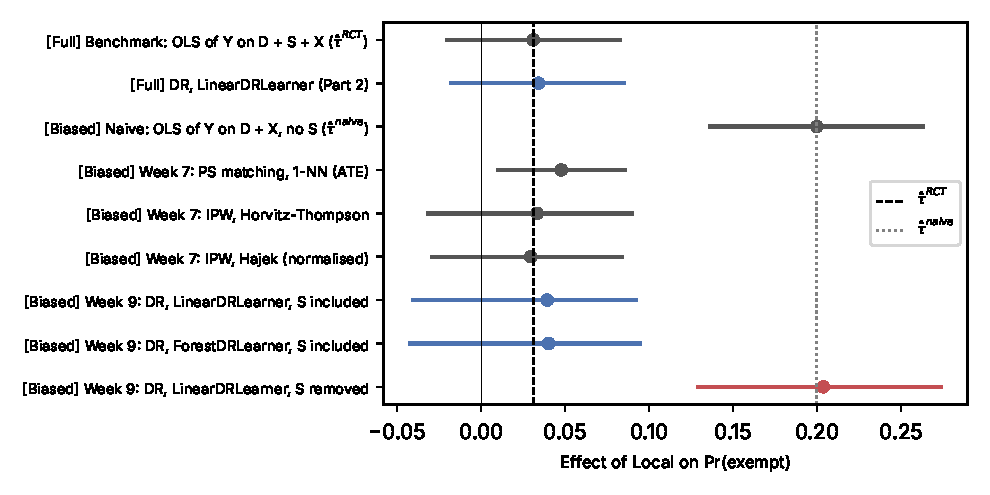
\includegraphics[width=0.82\linewidth]{figure2_estimates.pdf}
\caption{Point estimates and 95\% CIs from Table 3 (cluster or Abadie--Imbens SE $\times 1.96$ where there is no bootstrap CI). Blue: DR; red: DR with $S$ removed. Dashed: $\taurct$; dotted: $\taunaive$.}
\end{figure}
\begin{itemize}
\item \textbf{Result.} DR with $S$ gives 0.039 (95\% CI $[-0.041, 0.092]$) against $\taurct=0.031$ and $\taunaive=0.200$. It removes 95\% of the selection bias, and its CI contains $\taurct$ but not $\taunaive$.
\item \textbf{How the CIs are computed.} I resample whole neighbourhoods (the unit of randomisation) with replacement 200 times. In each draw I refit both cross-fitted nuisance models and the final stage, and I take the 2.5th and 97.5th percentiles of the 200 ATEs. Why 200: the Monte Carlo error of a bootstrap SE is about $\mathrm{SE}/\sqrt{2B}$, i.e.\ 5\% of the SE with $B=200$. That is enough for a CI, while each draw refits 11 models.
\item \textbf{Did DR beat IPW or matching? It beat matching (gap +0.008 vs +0.017) but not IPW (+0.002 for Horvitz--Thompson, $-0.001$ for Hajek).} I expected DR to do at least as well. AIPW adds an outcome model that corrects whatever the weights get wrong, and it is consistent if either model is right. Here, however, the weights get nothing wrong. Recipe B makes the true propensity score a logit in $S$, the logit is exactly what I fit, and Week 7 recovered $\hat\gamma=1.04$ against $\gamma=1$. So IPW is already consistent, and DR's insurance has nothing to insure against. The outcome model on its own (the plug-in $\frac1N\sum[\hat\mu_1-\hat\mu_0]$) gives 0.029, so both components are close to unbiased. The 0.006 gap between DR and IPW is about a fifth of one SE, which is finite-sample noise from fitting a second model. The two have the same bootstrap SE (0.031), so DR did not buy precision here either. DR's advantage would show up if the propensity model were misspecified (e.g.\ selection on a non-linear function of age); this design does not test that case.
\end{itemize}

\section{Doubly robust on the full experimental sample}
\textbf{Full sample, \texttt{LinearDRLearner}, same specification: ATE = 0.034 (bootstrap SE 0.027, 95\% CI $[-0.018, 0.085]$), vs $\taurct=0.031$ (SE 0.026).} In the experiment $D$ is random, so the estimated score is flat (0.42--0.54 in Week 7) and there is no selection to correct. The DR estimator returns the experimental answer, with essentially the same precision.

\section{Summary and conclusions}
\begin{itemize}
\item \textbf{Findings.} On the biased sample, all doubly robust learners give an ATE of 0.039--0.040, removing about 95\% of the 17-point selection bias. They agree with $\taurct=0.031$ within a third of a standard error, and the result does not change with the final stage or the nuisance learners. Removing $S$ sends the same estimators back to 0.204 $\approx\taunaive$. DR is only as good as the covariate set it is given, and the overlap plot cannot reveal the missing confounder. On the full sample DR returns 0.034, the experiment.
\item \textbf{Implications for the research question and Project 2.} (i) The substantive answer is unchanged across Weeks 6--9: chief collection raises exemptions by about 3 points, not significantly. Week 8 located this effect among owners aged 55+, the legally eligible. (ii) In the paper's Project Two table I will report the ``$S$ removed'' row next to the DR row: it is the clearest evidence that the methods work only because $S$ is observed. (iii) Since IPW and DR agree when the propensity score is correctly specified, a useful extension is to break it on purpose (e.g.\ fit the logit without $S^2$ while selecting on a non-linear function of age). This would show DR's advantage. (iv) For heterogeneity, I will move from the Week 8 meta-learners to the DR-learner CATE with cross-fitting and a BLP/GATES test, and apply it to the discretionary-exemption outcome.
\end{itemize}

\end{document}
